% This template has been tested with IEEEtran of 2015.
% !TEX options =  --shell-escape -synctex=1 -interaction=nonstopmode --aux-directory=aux -file-line-error "%DOC%"

% !TeX spellcheck = en-US
% !TeX encoding = utf8
% !TeX program = pdflatex
% !TeX TXS-program:compile = txs:///pdflatex/[--shell-escape]
% !BIB program = bibtex
% -*- coding:utf-8 mod:LaTeX -*-
% DO NOT DOWNLOAD IEEEtran.cls - Use the one of your LaTeX distribution
% For the final version, replace "draftcls" by "final"
\documentclass[journal,letterpaper]{IEEEtran}
\usepackage{preamble}
\begin{document}
% Enable following command if you need to typeset "IEEEpubid".
% See https://bytefreaks.net/tag/ieeeoverridecommandlockouts for details.
%\IEEEoverridecommandlockouts

\title{Proposal: Recognizing Pedestrian Behavior in Transit Crossings by Using Pose Estimation}

\author{%
  \IEEEauthorblockN{Sebastián Barrios Slight}\\
  \IEEEauthorblockA{sbarrios93@gmail.com}
}

% use for special paper notices
\IEEEspecialpapernotice{(XCS229II)}

% make the title area
\maketitle

% In case you want to add a copyright statement.
% Works only in the compsoc conference mode.
%
% Source: https://tex.stackexchange.com/a/325013/9075
%
% All possible solutions:
%  - https://tex.stackexchange.com/a/325013/9075
%  - https://tex.stackexchange.com/a/279134/9075
%  - https://tex.stackexchange.com/q/279789/9075 (TikZ)
%  - https://tex.stackexchange.com/a/200330/9075 - for non-compsocc papers

%%% ===============================================================================
\section{Introduction}\label{sec:introduction}
%%% ===============================================================================

As the development of autonomous vehicles (AVs) has increased dramatically in the past years, fueled by new technologies, but also for the hope of a safer transportation method, critical tasks have proven difficult to accomplish. A key challenge for advanced driver assistant systems (ADAS) and the design of truly AVs is to understand its environment and anticipate to actions of third parties on the road. Vulnerable Road Users (VRUs) behavior (e.g., pedestrians) is especially hard to predict, as most of the road rules don't apply to them, and their path can be considered more erratic than other road participants. Especially when driving at night or during adverse weather conditions, it becomes even more challenging due to the lack of visibility and increased uncertainty about others' behavior. 

%%% ===============================================================================
\section{Scope}\label{sec:scope}
%%% ===============================================================================
In this project, I will focus on trying to predict pedestrian intent of crossing by fitting a pose estimation skeleton to pedestrians and calculating the position of each key point of the skeleton to each other. The prediction will be made from the point of view of a decision-making vehicle (the \emph{ego} vehicle).

The input of the model will be frames of videos taken from a car where pedestrians can be seen at the sides of the road or performing some action (crossing, waiting to cross, etc.). The output will be the position of each pedestrian in the frame, and the probability that each pedestrian detected by the model is expecting to cross the road.

As the project is currently planned, there are two main steps to be accomplished.
\begin{itemize}
  \item[1.] \emph{Perform recognition of pedestrians in the video frames and fit a skeleton to their pose on the frame.} This is a critical part of the project, but the recognition of pedestrians and human pose estimation is not the main goal of the project. Being that the case, to achieve this step, an off-the-shelf model will be used. See \cite{SunXLW19} and \cite{DBLP:journals/corr/abs-1812-08008} for more details.
  \item[2.] \emph{Calculate the position of each key point of the skeleton with respect to one another and obtain the probability that the pedestrian is expecting to cross the road.} 
\end{itemize}

To test the accuracy of the model, a set of videos will be used to validate the model. After training the model will be fed with the test set, and the model will have to classify each pedestrian it encounters and calculate the probability that the pedestrian is expecting to cross the road. It is important to note that the model will also have to accurately recognize the pedestrians on the road, and the accuracy of the model will be penalized if the model does not perform well in this area. 
%
%%% ===============================================================================
\section{The Dataset}\label{sec:dataset}
%%% ===============================================================================
The main dataset for this project will be the Joint Attention in Autonomous Driving (JAAD) Dataset\footnote{\url{https://data.nvision2.eecs.yorku.ca/JAAD_dataset/}}. JAAD has been used in many of the papers published that relate to this project and is composed of 346 video clips recorded on board a vehicle, at 30 frames per second, that range from five to ten seconds long. The dataset comprises 82,302 frames (100\% of them have been annotated) and 2,786 pedestrians (of which 686 have annotations). The videos were recorded in a natural setting.

\begin{figure}[h]
  \centering
  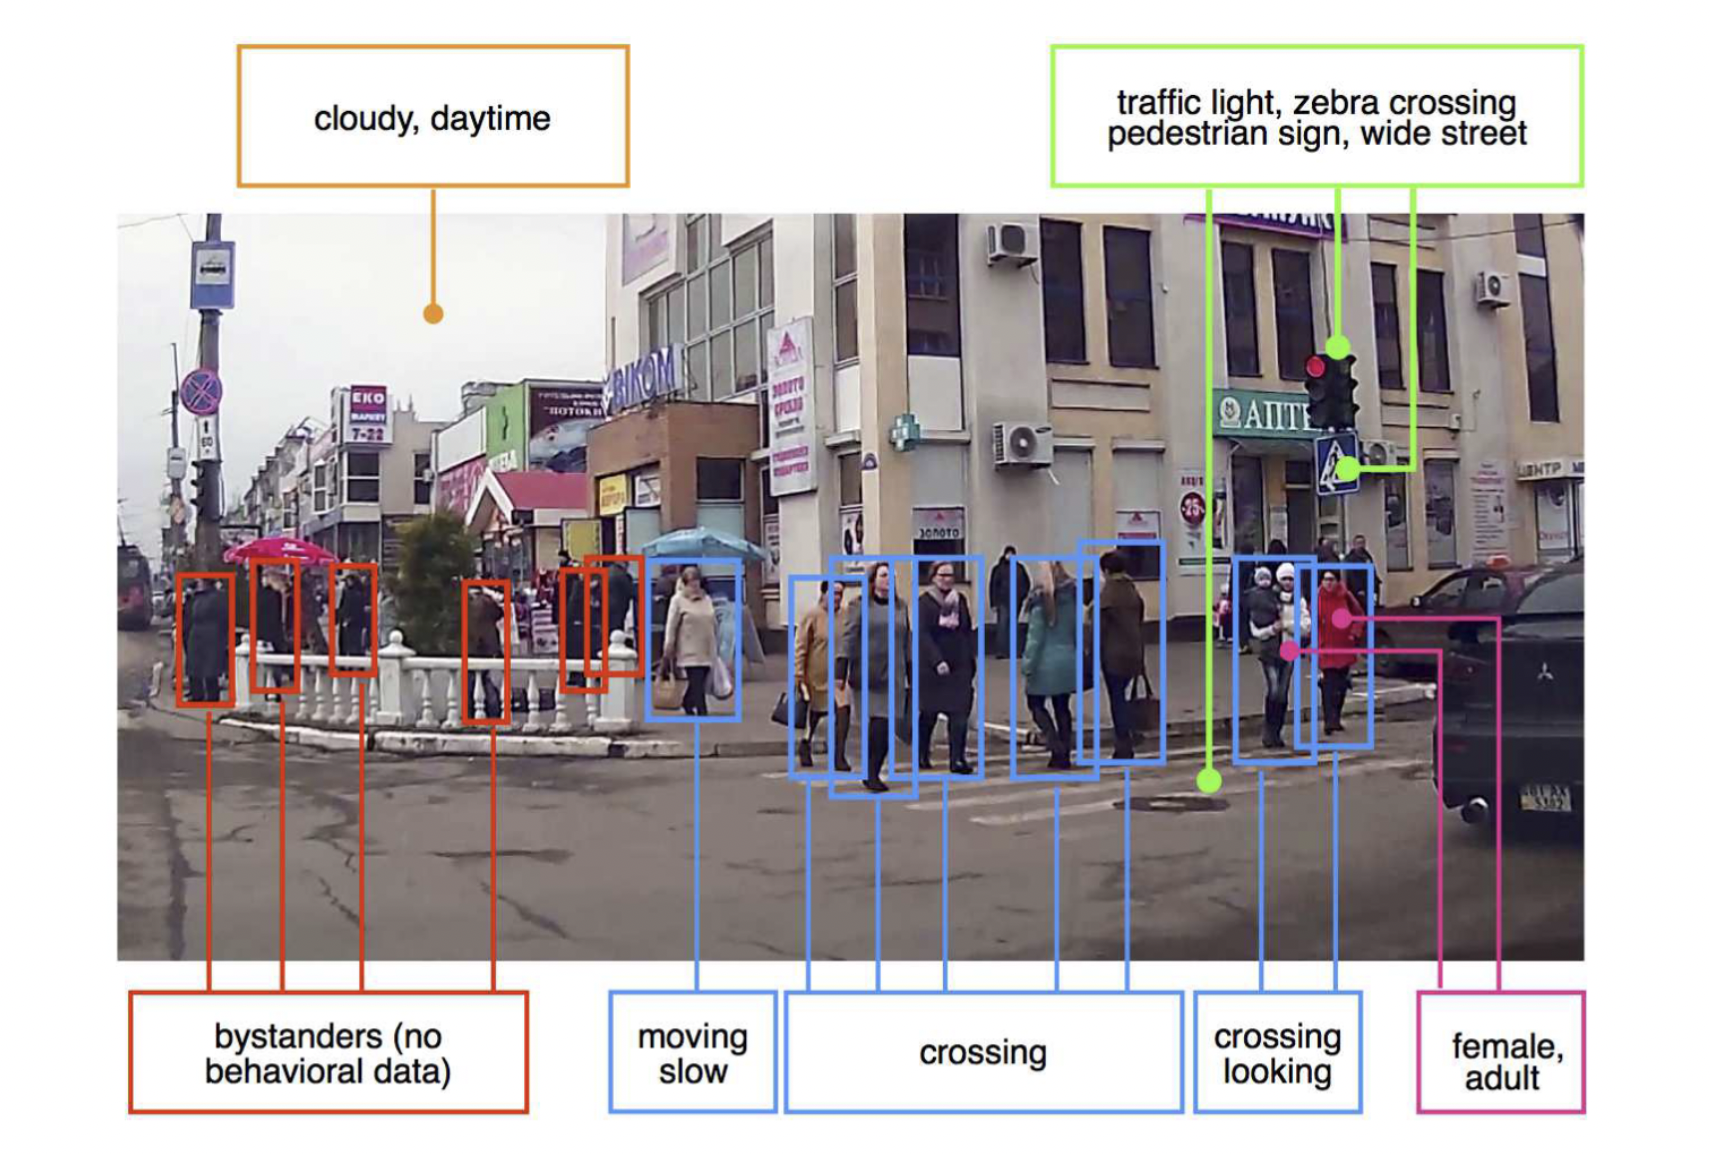
\includegraphics[width=.75\columnwidth]{figures/jaad-dataset.png}
  \caption{Example of annotated image of JAAD dataset (Originally published in \cite{rasouli2017ICCVW}).}
  \label{fig:dataset:jaad}
\end{figure}
%%% ===============================================================================
\section{Challenges Ahead}\label{sec:challenges}
%%% ===============================================================================
The main challenge of this project is to engineer the model in such a way that if there exists a correlation between the pose of a VRU and its intention to cross a road, the algorithm should be able to capture the information. Model selection will also play a critical role in achieving this.

Another challenge is deciding how many times the model should perform the prediction while a pedestrian stays inside the video frame. Because we already explained that VRU behavior can be unpredictable, the model will probably have to perform the prediction over the same individual multiple times. 

The model should also understand when a VRU has finished the task (i.e. finished crossing the road) to avoid the ego vehicle modifying its behavior because of subsequent actions performed by the VRU. 

Although it does not fall in the scope of this project, it is important to note that the behavior of the ego vehicle should not depend on whether the predicted value is over or under 50\%. Because a type II error (i.e., assuming a pedestrian will not cross when it actually is intending to cross) could result in a high human cost, the algorithm should be able to handle scenarios when there is not a strong prediction value. 
%%% ===============================================================================
%%% Bibliography
%%% ===============================================================================

% trigger a \newpage just before the given reference
% number - used to balance the columns on the last page
% adjust value as needed - may need to be readjusted if
% the document is modified later
%\IEEEtriggeratref{8}
% The "triggered" command can be changed if desired:
%\IEEEtriggercmd{\enlargethispage{-5in}}

% Enable to reduce spacing between bibitems (source: https://tex.stackexchange.com/a/25774)
% \def\IEEEbibitemsep{0pt plus .5pt}

\bibliographystyle{IEEEtranN} % IEEEtranN is the natbib compatible bst file
% argument is your BibTeX string definitions and bibliography database(s)
\bibliography{paper}

% Enfore empty line after bibliography
\ \\
%

%%% ===============================================================================
%\appendix
%\addcontentsline{toc}{chapter}{APPENDICES}

%\listoffigures
%\listoftables
%%% ===============================================================================

%%% ===============================================================================
%\section{My first appendix}\label{sec:appendix1}
%%% ===============================================================================

\end{document}

